% =====================================================================
%  jetportrait.tex -- Secs. 1.4.5-1.4.7.
%
%  Follows Ellis, Stirling & Webber (ESW), "QCD and Collider Physics",
%  Ch. 6 "Jet properties beyond fixed order" -- the chapter after the
%  one Secs. 1.4.1-1.4.4 are built on -- section for section:
%      1.4.5 Jet fragmentation  <-> ESW 6.1
%      1.4.6 Jet substructure    <-> ESW 6.4 + 6.5, extended with
%              Dokshitzer-Khoze-Mueller-Troyan (BPQCD) Sec. 9.2.
%  Supersedes qgjets.tex.
%
%  BIBTEX NEEDED in thesis.bib -- keys below are undefined until pasted.
%  ESW Ch. 5 (...1996d) is what Secs. 1.4.1-1.4.4 follow and is not
%  cited anywhere yet; it is offered here, not cited by this file.
%
%  @incollection{Ellis_Stirling_Webber_1996d,
%    author={Ellis, R. K. and Stirling, W. J. and Webber, B. R.},
%    title={Parton branching and jet simulation},
%    booktitle={QCD and Collider Physics},
%    series={Cambridge Monographs on Particle Physics, Nuclear Physics
%            and Cosmology},
%    publisher={Cambridge University Press}, address={Cambridge},
%    year={1996}, pages={157--192}}
%
%  @incollection{Ellis_Stirling_Webber_1996e,
%    author={Ellis, R. K. and Stirling, W. J. and Webber, B. R.},
%    title={Jet properties beyond fixed order},
%    booktitle={QCD and Collider Physics},
%    series={Cambridge Monographs on Particle Physics, Nuclear Physics
%            and Cosmology},
%    publisher={Cambridge University Press}, address={Cambridge},
%    year={1996}, pages={193--236}}
%
%  @book{Dokshitzer_Khoze_Mueller_Troyan_1991,
%    author={Dokshitzer, Yu. L. and Khoze, V. A. and Mueller, A. H.
%            and Troyan, S. I.},
%    title={Basics of Perturbative QCD},
%    publisher={Editions Fronti\`{e}res}, address={Gif-sur-Yvette},
%    year={1991}}
%
%  @article{Azimov_Dokshitzer_Khoze_Troyan_1985,
%    author={Azimov, Ya. I. and Dokshitzer, Yu. L. and Khoze, V. A.
%            and Troyan, S. I.},
%    title={Similarity of Parton and Hadron Spectra in {QCD} Jets},
%    journal={Z. Phys. C}, volume={27}, number={1}, pages={65--72},
%    year={1985}}
%
%  NOTATION -- ESW's throughout, so this reads on from 1.4.1-1.4.4:
%   D^h_i(x,t): subscript = initiating parton, superscript = observed.
%   The z^2 in eq:timelikeDglap is ESW (6.25) and is your own
%     eq:orderingCutoff; without it the small-x behaviour is wrong.
%   xi = ln(1/x), ESW (6.39).  (Hence no integrated-coupling xi; the one
%     place it is needed, eq:valenceSpectrum, uses a local w.)
%   ESW's b, from beta(a_s) = -b a_s^2, IS your beta_0 of eq:RGEquation,
%     and their a_s = 1/(b ln(s/L^2)) is your eq:runningCouplingLambda,
%     so eq:dlaMultiplicity is ESW (6.37) verbatim in your symbols.
%
%  ON beta_0 -- flagged, not touched.  Derivations are symbolic in
%  alpha_s = 1/(beta_0 ln(t/Lambda^2)) and hold whatever beta_0 is.  The
%  numbers (50/81, 2.4, 1/4) need 4 pi beta_0 = 11 - 2N_f/3, which is
%  also what ESW's b equals; intro.tex:178 carries an extra 4 pi
%  relative to the RGE at intro.tex:172 (beta_1 with (4pi)^4 is right).
%  BPQCD's b = 4 pi beta_0, hence the exponent of
%  eq:colorCurrentEvolution.  BPQCD (9.12) prints gamma there but their
%  (9.15) uses 50/81 = (50/9)/9, so gamma/(4 pi beta_0) is meant.
%  Signs in eq:multCollimationEq: <Q^2>_q/C_F = 1.8 - 0.8r and
%  <Q^2>_g/C_A = 0.8 + 0.2r; BPQCD (9.15) quotes both positive.
% =====================================================================

\subsection{Jet fragmentation}
\label{subsec:fragmentation}

A jet of energy \(E\) and opening angle \(\theta\) enters the cascade of
Sec.~\ref{sec:coherentPartonBranching} at its \emph{hardness}
\(\tilde{t}=E^2(1-\cos\theta)\simeq(E\theta)^2/2\); a cone of half-angle
\(\theta^\prime<\theta\) about its axis sits at \(\tilde{t}^\prime<\tilde{t}\) on the
same ladder, so narrowing the aperture and stopping the cascade early are one
operation. The \emph{fragmentation function} \(D^h_i(x,\tilde{t})\), the inclusive
probability of a hadron \(h\) with \(x=E_h/E_i\) in a jet opened by a parton \(i\),
evolves with the regularized Altarelli--Parisi kernels \(P_{ji}(z)\) --- the
\(\hat{P}_{ji}\) of Table~\ref{tab:splitfns} with their plus-prescription and
\(\delta(1-z)\) terms restored --- as
\begin{equation}
	\tilde{t}\frac{\partial}{\partial\tilde{t}}D^h_i(x,\tilde{t})
	= \sum_j\int_x^1\frac{dz}{z}\frac{\alpha_s}{2\pi}
	P_{ji}(z)\,D^h_j\!\left(\frac{x}{z}, z^2\tilde{t}\right) ,
	\label{eq:timelikeDglap}
\end{equation}
the \(z^2\) being Eq.~\ref{eq:orderingCutoff} and the only place coherence enters;
stopping at an intermediate scale gives the parton-level
\(D^j_i(x;\tilde{t},\tilde{t}^\prime)\). The first moment
\(\langle n_h\rangle_i=\int_0^1dx\,D^h_i\) diverges at lowest order, the moments of
\(P_{ji}\) being dominated by \(P_{gi}\to2\mathbf{Q}_i^2/z\); the \(z^2\)
regulates it, \(D\propto\tilde{t}^{\,\gamma}\) requiring
\(\gamma=\frac{\alpha_s}{2\pi}\int_0^1dz\,z^{\,j-1+2\gamma}P(z)\), so that
\begin{align}
	\gamma_{gg}(j,\alpha_s) &= \frac{1}{4}\left[
	\sqrt{(j-1)^2 + \frac{8C_A\alpha_s}{\pi}} - (j-1)\right]
	\;\xrightarrow[\;j\to1\;]{}\;
	\sqrt{\frac{C_A\alpha_s}{2\pi}} , \notag\\
	\langle n(\tilde{t})\rangle &\propto
	\exp\left[\int^{\tilde{t}}\gamma_{gg}(1,\alpha_s)
	\frac{d\tilde{t}^\prime}{\tilde{t}^\prime}\right]
	\propto
	\exp\left[\sqrt{\frac{2C_A}{\pi\beta_0}\ln\frac{\tilde{t}}{\Lambda^2}}\;\right] ,
	\label{eq:dlaMultiplicity}
\end{align}
a square root of \(\alpha_s\): the soft singularities are resummed, and
\(\langle n\rangle\) outgrows any power of \(\ln\tilde{t}\) while staying below any
power of \(\tilde{t}\). Keeping only these double logarithms is the
\emph{double-logarithmic approximation} (DLA), adding the next-to-leading ones the
\emph{modified leading-logarithmic approximation} (MLLA). Away from \(j=1\) the same
\(\gamma_{gg}\) gives a Gaussian in \(\xi\equiv\ln(1/x)\),
\begin{equation}
	x D^h_i \propto \exp\left[-\frac{(\xi-\xi_p)^2}{2\sigma^2}\right],
	\quad
	\xi_p = \frac{1}{4\beta_0\alpha_s(\tilde{t})}
	\simeq \frac{1}{4}\ln\frac{\tilde{t}}{\Lambda^2},
	\quad
	\sigma \propto \left[\ln\frac{\tilde{t}}{\Lambda^2}\right]^{3/4} ,
	\label{eq:humpBacked}
\end{equation}
the \emph{hump-backed plateau}~\cite{Azimov_Dokshitzer_Khoze_Troyan_1985}. A merely
kinematic cut-off at \(x\propto m/\sqrt{\tilde{t}}\) would put the peak at
\(\tfrac12\ln(\tilde{t}/\Lambda^2)\), twice the observed energy dependence: the soft
suppression is coherence.

\subsection{Jet substructure}
\label{subsec:substructure}

Every emission rate above is proportional to the emitter's squared colour charge, and
Eq.~\ref{eq:dlaMultiplicity} carries \(C_A\) whatever opened the jet, the cascade
being gluon-dominated after the first branching, so
\begin{equation}
	\frac{\mathbf{Q}_g^2}{\mathbf{Q}_q^2} = \frac{C_A}{C_F}
	= \frac{2N_c^2}{N_c^2-1} = \frac{9}{4} ,
	\qquad
	\langle n\rangle_i = \frac{\mathbf{Q}_i^2}{C_A}\langle n\rangle_g
	\;\Longrightarrow\;
	\frac{\langle n\rangle_g}{\langle n\rangle_q}
	\;\xrightarrow[\;\tilde{t}\to\infty\;]{}\;\frac{C_A}{C_F} .
	\label{eq:casimirRatio}
\end{equation}
The second moment is reduced likewise, widening a gluon jet's multiplicity
distribution by \(\sqrt{C_A/C_F}\), while in the spectrum the peak \(\xi_p\) is common
to both and only its height differs, as \(C_F:C_A\). For the angular size the
Sterman--Weinberg criterion, all but a fraction \(\epsilon\) of the energy inside a
half-angle \(\delta\), gives at fixed \(f_2,\epsilon\)
\begin{align}
	f_2 &= 1 - \frac{4\alpha_s\mathbf{Q}_i^2}{\pi}
	\ln\frac{1}{\epsilon}\ln\frac{1}{\delta} , \notag\\
	\delta_q &\sim \exp\left[\frac{\pi(1-f_2)}
	{4C_F\alpha_s(\tilde{t})\ln\epsilon}\right] ,
	\qquad
	\delta_g \sim \delta_q^{\,C_F/C_A} = \delta_q^{\,4/9} ,
	\label{eq:swWidth}
\end{align}
the charge in the denominator leaving the gluon jet the wider. Both ratios are
asymptotic: energy conservation and MLLA corrections bring the multiplicity ratio to
\(\simeq1.5\) at present energies.

Energy and multiplicity are not collimated alike. A cone \(\theta^\prime\) intercepts
the cascade at \(\tilde{t}^\prime\) (Eq.~\ref{eq:angularOrdering}), so the energy it
holds follows \(\sum_jD^j_i(z;\tilde{t},\tilde{t}^\prime)\); at \(z\to1\) the valence
term dominates and the \(z\to1\) singularity of \(P_{ii}\), exponentiated as in
Sec.~\ref{subsec:dglap}, gives \(D^i_i\propto(1-z)^{-1+4\mathbf{Q}_i^2w}\),
\(w=\int_{\tilde{t}^\prime}^{\tilde{t}}
(d\tilde{t}^{\prime\prime}/2\tilde{t}^{\prime\prime})(\alpha_s/2\pi)\), which falls at
both ends and peaks at
\begin{equation}
	\frac{\theta_z}{\theta} =
	\left(\frac{\sqrt{\tilde{t}}}{\Lambda}\right)^{-\gamma_E(z)},
	\qquad
	\begin{array}{r|cc}
		z & \gamma_E^{\,q}(z) & \gamma_E^{\,g}(z) \\ \hline
		0.9 & 0.55 & 0.30 \\
		0.5 & 0.83 & 0.54
	\end{array}
	\label{eq:energyCollimation}
\end{equation}
--- a power of the hardness, faster for quark jets, as in Eq.~\ref{eq:swWidth}. The
particles in that cone instead correlate the flux with one particle in it: convolving
\(D^j_i(z;\tilde{t},z^2\tilde{t}^\prime)\) with \(D^h_j(x/z,z^2\tilde{t}^\prime)\) at
\(x\ll1\), where Eq.~\ref{eq:humpBacked} is insensitive to the energy balance, gives
\(\langle n_h\rangle_i=(\langle\mathbf{Q}^2\rangle_i/C_A)\langle n_h\rangle_g\) with
\(\langle\mathbf{Q}^2\rangle_i=\langle z_g\rangle_iC_A+\langle z_q\rangle_iC_F\), the
\emph{average colour current} of the partons caught. Inside a cone every jet is a
gluon jet, and \(\langle\mathbf{Q}^2\rangle_{q,g}\to2.4\) as \(\theta^\prime\to0\), so
the \(9/4\) of Eq.~\ref{eq:casimirRatio} tends to \(1\) for a narrow cone at any
energy. Repeating for particles leaves a colour ratio between \(1\) and
\(\simeq1.8\), so Eq.~\ref{eq:dlaMultiplicity} alone fixes
\begin{equation}
	\theta_\delta \sim \theta\,
	\langle n(\tilde{t})\rangle^{-(\pi\beta_0/2C_A)\ln(1/\delta)} ,
	\qquad
	\frac{\pi\beta_0}{2C_A}\ln 2 \simeq 0.26 \simeq \frac{1}{4} .
	\label{eq:multCollimation}
\end{equation}
\(\langle n\rangle\) growing only as the exponential of a square root,
\(\theta_\delta\) falls slower than any power of the hardness where \(\theta_z\) falls
as a power (Fig.~\ref{fig:collimationCones}): a narrow core of energy in a broad halo
of particles, separating as the jet hardens.

\begin{figure}[htbp]
	\centering
	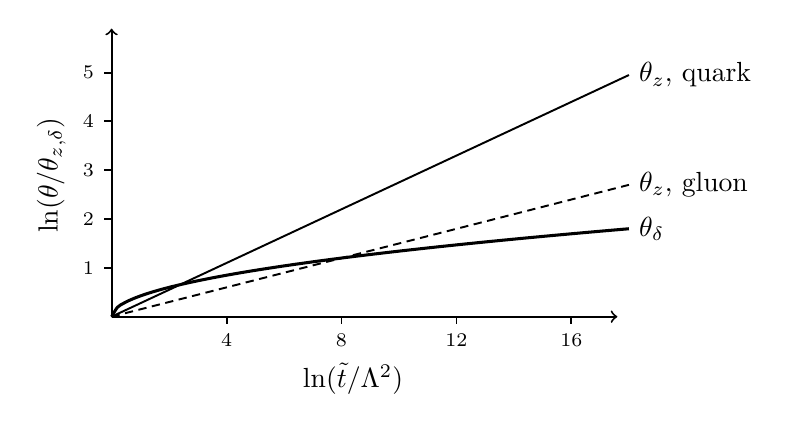
\begin{tikzpicture}[x=0.365cm, y=0.62cm, line width=0.7pt]
		\draw[->] (0,0) -- (17.6,0);
		\draw[->] (0,0) -- (0,5.9);
		\foreach \i in {4,8,12,16} {
			\draw (\i,0) -- (\i,-0.14) node[below] {\scriptsize\(\i\)};
		}
		\foreach \j in {1,2,3,4,5} {
			\draw (0,\j) -- (-0.26,\j) node[left] {\scriptsize\(\j\)};
		}
		\node[below] at (8.4,-0.75) {\(\ln(\tilde{t}/\Lambda^2)\)};
		\node[rotate=90] at (-2.1,2.9) {\(\ln(\theta/\theta_{z,\delta})\)};
		\draw[domain=0:18, samples=2] plot (\x, {0.275*\x});
		\draw[domain=0:18, samples=2, densely dashed] plot (\x, {0.150*\x});
		\draw[domain=0:18, samples=90, smooth, line width=1.1pt]
		plot (\x, {0.4245*sqrt(\x)});
		\node[right] at (18,4.95) {\(\theta_z\), quark};
		\node[right] at (18,2.70) {\(\theta_z\), gluon};
		\node[right] at (18,1.80) {\(\theta_\delta\)};
	\end{tikzpicture}
	\caption[Collimation of the energy and multiplicity flows of a jet]{%
		Collimation of the energy and of the multiplicity flow of a jet against its
		hardness, for \(z=0.9\), \(\delta=\tfrac12\), \(N_f=3\). The energy cone
		\(\theta_z\) of Eq.~\ref{eq:energyCollimation} closes linearly in
		\(\ln(\tilde{t}/\Lambda^2)\) and faster for quark jets; the multiplicity cone
		\(\theta_\delta\) of Eq.~\ref{eq:multCollimation} only as its square root.}
	\label{fig:collimationCones}
\end{figure}


The angularities of Chapter~\ref{ch:angularities} replace the cone by a weight, and
the same cascade fixes their distributions:
\begin{align}
	\lambda_\beta^\kappa &= \sum_{c\,\in J} z_c^\kappa
	\left(\frac{\Delta R_c}{R}\right)^{\beta} ,
	\qquad
	z_c = p_{\mathrm{T},c}\Big/\!\!\sum_{c^\prime\in J}p_{\mathrm{T},c^\prime} ,
	\notag\\
	dn &= \frac{2\alpha_s\mathbf{Q}_i^2}{\pi}\frac{dz}{z}\frac{d\theta}{\theta}
	= \frac{2\alpha_s\mathbf{Q}_i^2}{\pi}\,du\,dv ,
	\qquad
	u = \ln\frac{1}{z} , \qquad v = \ln\frac{R}{\theta} ,
	\label{eq:angularityDef}
\end{align}
the density being the single-emitter antenna pattern of
Eq.~\ref{eq:antennaSplitXSec} with \(\zeta\simeq\theta^2/2\), uniform on the quadrant,
each emission contributing \(z^\kappa(\theta/R)^\beta\) to the sum, which at this
accuracy is dominated by one of them. Let \(\Sigma_i(\lambda)\) be the fraction of
jets whose angularity falls below a value \(\lambda\). At \(\kappa=1\) an emission
carries \(\lambda^1_\beta\) above \(\lambda\) when \(u+\beta v<\ln(1/\lambda)\), a
triangle of area \(\ln^2(1/\lambda)/2\beta\), and vetoing every such emission gives
\begin{equation}
	\Sigma_i(\lambda) = \exp\left[-\frac{\alpha_s\mathbf{Q}_i^2}{\pi\beta}
	\ln^2\frac{1}{\lambda}\right] ,
	\qquad
	\Sigma_g(\lambda) = \left[\Sigma_q(\lambda)\right]^{C_A/C_F} ,
	\label{eq:angularitySudakov}
\end{equation}
a Sudakov form factor vetoing an observable rather than a cone, and at \(\beta=1\) the
double-logarithmic thrust distribution~\cite{Ellis_Stirling_Webber_1996e}. Equations~\ref{eq:swWidth} and
\ref{eq:angularitySudakov} invert one another. At \(\kappa=0\) the vetoed region is
instead the strip \(v<\ln(1/\lambda)/\beta\), unbounded in \(u\): nothing
exponentiates and \(\lambda^0_\beta\) counts emissions, governed by
Eq.~\ref{eq:dlaMultiplicity}. So \(\lambda^1_1\) is the jet width and measures
\(\theta_z\), \(\lambda^0_0\) the jet multiplicity and \(\theta_\delta\), and
\((\kappa,\beta)\) carries one into the other --- with the quark--gluon memory at
large \(u\), small \(v\), exactly where grooming cuts, so the quark and gluon
fractions of a sample must be fixed before a change in its angular structure is read
as a medium effect.
